\chapter{Introduction}

Most of the Internet traffic is content, and most of the Internet connected hosts are mobile. A key example of the content-dominated nature of the Internet is that online video alone accounts for nearly 67\% of traffic today and is expected to grow to nearly 80\% by 2018 \cite{cisco-videogrowth}. The evidence of a highly mobile Internet is that close to 5 billion mobile devices connect to the Intenet today and they generate more traffic than wired devices \cite{cisco-vni}.

%It is estimated that a vast majority of network traffic on the Internet is content, with videos alone expected to account for 80\% of all traffic by 2018 . By 2020, the number of Internet connected mobile end hosts is expected to grow to nearly 10 billion and the total traffic originated by mobiles is poised to approach that by wired devices .

A content-dominated, highly mobile Internet needs several forms of infrastructure support. It needs network switches and links with sufficient capacity to carry traffic to end users. It needs servers to sustain and accelerate delivery of content. It also needs  infrastructure to help establish and maintain connections in the presence of high network mobility (or changing of addresses) of connection end-points. The focus of this thesis is to design \emph{services} that manage the resources on such infrastructures towards achieving their desired goals.

%the design of services that manage the infrastructure resources achieve the desired goals.
%This thesis focuses on the design of services that manage the infrastructure resources achieve the desired goals.

%The focus of this thesis is the design of these infrastructure 

%In the presence of frequent network mobility or changing addresses, infrastructure support becomes necessary for . This thesis focuses on the design of services that manage the infrastructure resources achieve the desired goals.

\section{Infrastructure characteristics}
%	Characteristics of infrastructure}

Our service designs are strongly influenced by the following characteristics of the infrastructures that support a content-dominated, highly mobile Internet.

\textbf{Cost-intensive} There is a substantial captial and operational cost in running a large-scale infrastructure \cite{greenberg2008cost}, and which causes a sigificant reduction in the profit margins of the infrastructure owner. A prominent example of cost-intensive, low-profit infrastructures are Internet service provider (ISP) networks \cite{isp-low-profit}. Thus, a main goal of service design is to reduce cost while meeting performance and other constraints. 

\textbf{Geo-distributed:} These infrastructures are often highly geo-distributed, e.g., a large ISP or a content delivery network (CDN) has Points-of-Presence  at hundreds of locations \cite{dilley2002globally}. Thus, it is necessary that services be designed to leverage geo-distributed deployments for reducing user-perceived latencies.

\textbf{Locality-exhibiting workload:} Real-world workloads served by these infrastructures tend to exhibit significant geographic and temporal locality \cite{NCDN, youtubeUGC, vodP2Pbenefit, cellularvideotraffic}. Exploiting locality of demand to reduce infrastructure cost as well as user-perceived latencies is a key focus in our service designs.

\section{Degrees of freedom in infrastructure service design} 

Due to a geo-distributed infrastructure deployment, infrastructure services commonly make three sets of decisions: \emph{content placement}, \emph{request redirection}, and \emph{network routing}. As each of these decisions can be made relatively independent of others, we call them ``degrees of freedom'' available to a service.

\begin{itemize}
	\item
	\textbf{Content placement} selects the locations at which a content is placed. Its objective  is to balance resource cost of keeping multiple content replicas with the benefits of improved availability and reduced user-perceived latency.
	\item
	\textbf{Request redirection} selects a location to send a request to, with a preference for selecting a location that is nearby and has sufficient resources to serve the request.
	\item
	\textbf{Network routing} (or \textbf{traffic engineering}) selects the physical paths between nodes in the network based on topoology and traffic demand patterns. A key goal is to avoid congestion hotspots in the network.
\end{itemize}


\section{Thesis statement}



\emph{Content placement is a powerful factor, and is often more powerful than redirection and routing, in determining the cost, performance and energy-related metrics for infrastructures supporting a content-dominated, highly mobile Internet.}



\section{Why placement is more powerful than redirection, routing}

Geo-distributed infrastructure and workload locality makes content placement a powerful degree of freedom. Workload locality implies that a content is typically popular in only a few regions at any given time, and as a result only a few replicas of a content placed in those regions  are sufficient to reduce user-perceived latency for most users. Further, the geo-distributed infrastructure enables these few replicas to be placed close to regions of demand, thereby achieving a good tradeoff between user-perceived latency and cost of content replication. We illustrate with a couple of examples why placement can be a more powerful degree of freedom than redirection and routing in designing infrastructure services.


\begin{figure}
	
	\centering
	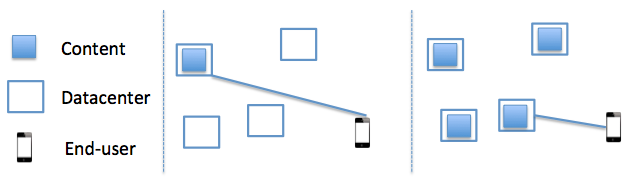
\includegraphics[scale=0.5]{fig/placement-vs-redirection.png}
	\caption{Placement vs. redirection: Content placement creates options for the redirection scheme to choose a nearby location for reducing user-perceived latencies.}	
	\label{fig:placement-redirection}
\end{figure}


\textbf{Placement vs. redirection:} Suppose a user requests a content that is placed only at a remote location as in Figure \ref{fig:placement-redirection} (left). Irrespective of the redirection scheme, a user will observe high latencies to fetch content from the remote location. Placement is more powerful that redirection becasue it can create more options for the redirection scheme, enabling it to choose a location that is nearby as shown in Figure \ref{fig:placement-redirection} (right). Thus, effective placement is a pre-requisite for a redirection scheme to provide low latencies.


%We briefly explain the \emph{traffic engineering} problem that is pertinent to our discussion of placement vs. routing. Traffic engineering computes network routing based on inputs of are the network topology, link capacities, and a \emph{traffic matrix}. A traffic engineering scheme computes routing to satisfy traffic demands while optimizing a cost function dependent on link utilization. For example, a common cost function is the maximum link utilization, MLU \cite{rexford}. 


\textbf{Placement vs. routing:} Content placement is more powerful than routing because it can change the \emph{traffic matrix} for which the routing is to be computed. A traffic matrix is a 2-dimensional matrix representing the demand in the network. The $i,j$-th entry in this matrix is the traffic from node $i$ to node $j$ in the network topology \cite{fortz2000internet}.  Let us take an example traffic matrix for which routing is to be computed (Figure \ref{fig:placement-routing}). Content placement can turn any traffic matrix into a null matrix (one whose all entries are zero) provided all content that a node in a network needs is placed at the same node. Such a placement obviates sending traffic to any other node, and therefore makes routing a trivial problem. While this is an extreme example, and one may not have sufficient resources to place content at all locations in the network, it demonstrates that the ability to change the traffic matrix makes content placement more powerful than routing.

\begin{figure}
	\centering
	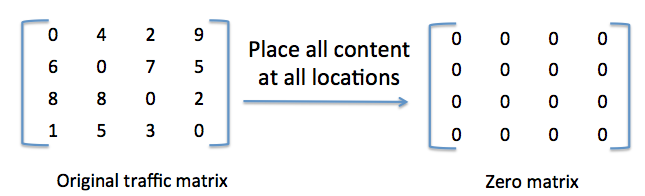
\includegraphics[scale=0.4]{fig/placement-vs-routing.png}
	\caption{Placement vs. routing: content placement is more powerful than routing since it can change the  traffic matrix itself.}
	\label{fig:placement-routing}
\end{figure}

\section{Research overview}

We study the design of services for the following infrastructures in this thesis.

\begin{description}
	\item[Internet service provider (ISP):] ISPs perform traffic engineering to achieve several objectives such as cost and congestion reduction, fault tolerance etc. As we explain in Section \ref{sec:intro-te}, our work designs and evaluates traffic engineering in content-dominated ISP networks while accounting for its interaction with placement and redirection schemes. 
	\item[Global name service (GNS):] GNS can enable establishing and maintaining connections between mobile entities on the Internet. As we explain in Section \ref{sec:intro-gns}, our name service design, Auspice, meets the challenge posed by high mobility, which is to return up to date addresses for billions of mobile names with frequently changing network address.
	\item[Content datacenter (CDC):] Content datacenters are used to cache and serve content to end users. As we explain in Section \ref{sec:intro-cdc}, our work quantifies the tradeoff between user-perceived performance and energy savings achieved via a coordinated consolidation of servers and switches, and presents the design and implementation of a system to leverage this tradeoff.
\end{description}

\subsection{Traffic engineering in content-dominated ISP networks}
\label{sec:intro-te}
In an ISP network with content-dominated traffic, traffic engineering decisions that compute network-layer routing are not isolated from traffic adaptation occuring at application-layer. For example, content placement and request redirection determine the traffic matrix and hence influence traffic engineering. While the interaction between network routing and application adaptation has been studied previously \cite{Roughgarden,selfishQiu,Jiang2009,JohariGameTheory, CATE, P4P}, the distinguishing aspect of our work it to study the role of placement strategies on this interaction.

We design and evaluate traffic engineering schemes in two scenarios that vary in terms of the flexibility of content placement. The first scenario is a more common occurence in the present day Internet, in which an ISP has little control over placement and redirection. The second scenario is motivated by a recent, potentialy transformative trend: Network CDNs (NCDNs) -- CDNs deployed by ISPs on their infrastructures. Unlike traditional ISPs, NCDNs enjoy full control over placement, redirection and routing on their networks.

\subsubsection{ISP network with content location diversity}

We model a content-dominated ISP network by accounting for its \emph{location diversity} -- the presence of content at multiple network locations, and the ability of end users to download content from those locations. Location diversity is enabled by several types of applications and services, such as CDNs, P2P applications, mirrored websites. We create location diversity using a simple content placement scheme -- randomly placing content at multiple locations --, to reflect the limited control of ISPs on content placement in their networks. 

%We further assume that users can download content in parallel from all locations. 

Our work presents an experimental comparison of several classes of traffic engineering schemes using data from real ISP topologies and traffic matrices. A key finding is that accounting for the application adaptation to location diversity increases the capacity achieved by several state-of-the-art traffic engineering schemes, and, surprisingly, blurs the capacity achieved by them. Here, capacity refers to the ability of a traffic engineering scheme to tolerate an increase in traffic demand. Even a static shortest-path routing, or in other words a ``no'' traffic engineering  scheme is at most 30\% sub-optimal in terms of capacity. Overall, these results suggest that even a limited placement flexibility reduces the value of carefully engineering routing. The value of traffic engineering is further reduced in an NCDN where the content placement flexibility is even greater.

\subsubsection{Network CDNs}

There are strong economic factors motivating ISPs to transform into NCDNs for delivering content to users on its network: need for additional revenue source in the face of falling bandwidth prices due to competition and technology trends, viability of monetizing NCDNs by selling content-based services to end users, easy availability of CDN technology in the form of licensed and managed CDNs and reduction in backbone traffic due to content caching via NCDNs \cite{telco-cdn-arguments}. These factors have motivated more than 30 ISPs to deploy NCDNs on their network.

NCDNs represent a paradigm shift in which both content delivery and traffic engineering is handled by a single entity. This change affects the metrics of interest of an NCDN as well the techniques it can use. While a traditional ISP is concerened with traffic enginerring related objectives such as network link utilization, and a traditional CDN is concered with optimizing user-perceived performance, an NCDN is concered with both these metrics. While a traditional ISP can decide network routing and a traditional CDN can decide placement and redirection, but only an NCDN can decide placement, redirection and routing. Besides using existing techniques to handle these tasks independently, an NCDN also has the option of optimizing these decisions jointly. 

Our contribution is to evaluate existing schemes as well as a new joint optimization scheme for NCDNs based on real network topologies and extensive real world content access traces from Akamai CDN. The schemes we evaluate include (1) a simple caching scheme for placement and a static-shortest path routing, (2) a joint optimization based on historic demand patterns and (3) an ideal joint optimization with future knowledge of content demand. Of particular interest to NCDNs are demand-oblivious schemes such as the first scheme, as they make placement and routing decisions without measurement of content demand and simplify network management for the operators.

Our main finding is that the simple demand oblivious scheme is effective in improving network and latency cost for an NCDN: it performs signficantly better than  the history-based joint optimization scheme and performs close to the ideal-joint optimization scheme. The history-based joint optimization scheme suffers due to poor placement for workloads with poor predictability of content demand and sigificant daily churn. The demand-oblivious scheme performs well largely due to its placement scheme, which achieves high cache hit rates from caches placed inside the network. We also show that the demand-oblivious scheme can gain only a small ($< 10\%$) cost reduction by using traffic engineering instead of a static-shortest path routing. Overall, our findings question the value of traditional traffic engineering for NCDNs and simplify the task of managing NCDNs.

\subsection{Global name service for a highly mobile Internet}
\label{sec:intro-gns}


The Internet has a poor support for estabilishing and maintain connections between mobile entities. Today, it is difficult to initiate a connection with a mobile device since there is no global infrastructure to locate it. As a result, mobile communication initiation is mostly unidirectional in the Internet, from the mobile to the fixed hosts. The lack of this basic functionalily has led to application-specific solutions which causes both redundant effort by developers and possibly redundant infrastructure expenditure also. Yet, support for mobility is patchy among applications: SSH sessions terminate unexpectedly, HTTP downloads terminate before completion and VoIP calls get disrupted when network addresses change.

A key reason for the Internet's poor support for moblity is that communication on the Internet is based on IP addresses that keep changing due to mobility. On the other hand, what remains unchanged is the name or the identity of communication end-points. Thus a \emph{name-based communication} paradigm is a promising solution to mobilty. A  global name service (GNS) can enable such a name-based communication by maintaining an up-to-date mapping from names to network addresses for all names. 

Figure \ref{fig:gns-example} illustrates how a GNS helps establish connections in a common network mobility scenario. A mobile user Bob changes its network address and updates the GNS with its new address soon after. Afterwards, another mobile user Alice obtains Bob's new address from the GNS and is able to establish connection with Bob despite Bob's mobilty.

\begin{figure}
	\centering
	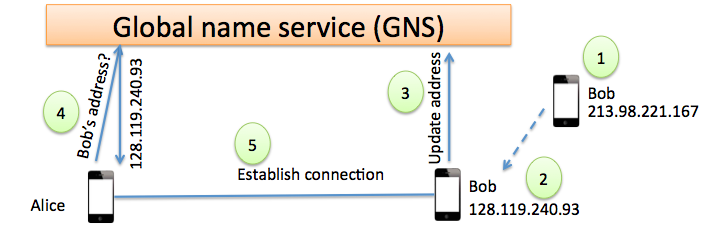
\includegraphics[scale=0.4]{fig/gns-example.png}
	\label{fig:gns-example}
	\caption{A global name service helps establish and maintain connections between mobile entities by keeping an up-to-date mapping from their names to their network addresses.}
\end{figure}

To appreciate the challenges in implementing such a GNS, we discuss the limitations of the Internet's existing naming service DNS as a solution for mobility.
\begin{description}
	\item[Passive caching:] 
	DNS relies heavily on passive caching based on TTLs for reducing both system load and user-perceived latency. However, high mobility severely limits effectiveness of TTL-caching. Establishing connection under high mobility requires up-to-date knowledge of network addresses, that must be obtained from \emph{authoritative name services} in DNS. So, the load and the user-perceived latency increase with the mobility rate irrespective of the TTL.
	\item[Static placement:] 
	Under high mobility, the latency to an authoritative name service determines user-perceived request latency in the common case. Today, authoritative name service locations are chosen statically irrespective of where the request demand is coming from, which could result in highly sub-optimal request latencies for users requesting the name service from a location distant from the statically placed replicas. 
	\item[Hierarchical names:]
	DNS uses a hierarchical design of namespace as well as federation structure. Due to DNS's hierarchical design, the main proposal to enhance DNS's security, DNSSEC, is dependent on a single root of trust. 
\end{description}

While the first two problems are related to authoritative name services and can be addressed within the scope of current DNS, the third issue requires a clean slate redesign of the naming system.   Below, we discuss our naming system and authoritative name service designs.
\begin{description}
	\item[Global naming system:] Our global naming system improves upon DNS's design in two aspects. First, it supports multiple roots of trust as a part of the naming system, thereby addressing the single root of trust problem in DNS. Second, it supports name-to-address resolution for arbitrary names unlike DNS, which restricts names to be hierarchical. In doing so, our naming system gives applications the full flexibility in choosing names. 
	\item[Auspice:] Our name resolution service, Auspice, resolves names to their network addresses, both represented in any format, under high mobility. The flexibility of name and address formats makes Auspice deployable in the Internet today as a scalable authoritative name service, potentially enhacing support for mobility in the present day Internet as well. 
\end{description}

A key distinction betweeen Auspice and existing name services is Auspice's \emph{demand-aware placement} of name records. Name records store name-to-address mapping as well other attributes. Auspice's demand-aware placement heuristic adapts the set of replicas for a name record based on read-to-write ratios, overall system load and the geo-distribution of demand for a name record to provide low latency name-to-address lookups in a cost-effective manner. Auspice' placement enables it to significantly outperform commercial managed DNS services, DHT-based name service designs as well as static placement schemes such as random-$k$ and replicate-all. This finding demonstrates the importance of placement in Auspice's design.

% that follow same the request redirection scheme as Auspice -- nearest replica routing based on measured network latencies. This finding demonstrates the importance of placement over redirection in Auspice's design.

\subsection{Energy optimization in content datacenters}
\label{sec:intro-cdc}

In today's content-dominated Internet, it is not surprising that datacenters and Points-of-Presence (PoPs) are dedicated to storing and serving content to end users. We call these datacenters and PoPs {\em content datacenters} (or, \cdc s). The three degrees of freedom -- placement, redirection and routing -- discussed in a wide-area setting previously, are also available inside a \cdc: content placement to select which servers to store on content on, request redirection to select which server inside a \cdc\ to send a request to, and network routing on \cdc\ topology. 

Energy use is a key concern for \cdc\ operator, e.g., Akamai CDN, managing a large global network of \cdc's, which can comprise of 100K servers or even more. A potential approach to reduce energy is \emph{consolidation} in a \cdc. Consolidation of servers, which uses only a fraction \cdc\ servers for placement and redirection and turns remaining servers off, can reduce server energy use. Consolidation of network, which routes network traffic via only a fraction of switches and links and turns remaining switches and links off, can reduce network energy use. A key concern for operators seeking to deploy these techniques is to understand the tradeoff between energy use and performance, i.e., do energy saving benefits outweigh the performance penalty incurred?

Our work presents the first quantitative analysis of energy-performance tradeoff for a \cdc\ based on a real \cdc\ workload and present the design and implementation of a system, \shrink, to leverage this tradeoff. A key insight, supported via experiments, is that cache hit rates, despite server consolidation, remain close to an unconsolidated datacenter. A small reduction in hit rate helps mitigate the impact of consolidation on user-perceived latency. This finding is explained by the skewed content popularity obseved in real workloads, due to which working set size of content remains small compared to the storage available in a CDC. Our quantitative analysis shows that \shrink\ reduces energy use by 35\% over a baseline scheme that keeps entire datacenter always on while increasing the mean, 95-th \%-ile and 99-th \%-ile latencies by 8\%, 3\% and 15\% respectively. 

While previous work has studied server and network consolidation in isolation, we show that a coordinated approach for server and network consolidation reduces \emph{network} energy use more than otherwise possible. We consider a simple \emph{network-aware server consolidation} scheme that selects the active servers in a left-to-right order in a topology. The same network consolidation scheme results in up to 42\% less network energy use when used with our network-aware server consolidation instead of a network-unaware server consolidation scheme that selects servers randomly. 

Our results show that placement affects both server and network energy use in a \cdc. Due to an effective placement, cache hit rates remain high despite consolidation, which helps reduce server energy use with a modest performance impact. Further, our network-aware server consolidation is able to significantly reduce network energy use over a network-unaware server consolidation by coordinating the placement and redirection with the routing in a \cdc. These results further support our statement that content placement is of key importance in a content-dominated Internet.


\section{Thesis organization}

The thesis comprises of three parts that correspond to our three research topics.

In the first part, which includes Chapter \ref{ch:te-background}, Chapter \ref{ch:beyondmlu} and Chapter \ref{ch:ncdn}, we present our research on traffic engineering in content-dominated ISP networks. Chapter \ref{ch:te-background} presents background on traffic engineering, content delivery and the interaction between traffic engineering and application-layer adaptation, and motivates the key research questions we address on this topic. Chapter \ref{ch:beyondmlu} presents a comparison of traffic engineering schemes in a network with location diversity of content. Chapter \ref{ch:ncdn} designs and evaluates traffic engineering and content delivery schemes in a Network CDN.

The second part, which includes Chapter \ref{ch:intro-auspice}, presents the design, implementation and evaluation of Auspice -- a global name service for a highly mobile Internet.

The second part, which includes Chapter \ref{ch:shrink}, presents the design, implementaiton and evaluation of Shrink - a system for reducing energy use of content datacenters via a coordinated consolidation of servers and switches.

\section{Previous publications and collaboration}

\textbf{Chapter \ref{ch:beyondmlu}} revises a previous publication: A. Sharma, A. Mishra, V. Kumar, A. Venkataramani. Beyond MLU: An Application-Centric Comparison of Traffic Engineering Schemes. \emph{Proc. IEEE INFOCOM, April 2011}. Aditya Mishra and Vikas Kumar provided invaluable support in performing experiments for this work.

\textbf{Chapter \ref{ch:ncdn}} revises a previous publication: A. Sharma, A. Venkataramani, R. Sitaraman. Distributing Content Simplifies ISP Traffic Engineering. \emph{Proc. ACM SIGMETRICS, June 2013}. Ramesh Sitaraman provided access to Akamai datasets for this work. A realistic experimental evaluation would not have been possible without these datasets.

\textbf{Chapter \ref{ch:intro-auspice}} revises a previous publication: A. Sharma, X. Tie, H. Uppal, D. Westbrook, A. Venkataramani, A. Yadav. A Global Name Service for a Highly Mobile Internetwork. \emph{Proc. ACM SIGCOMM, August 2014}. 
This work also appears in Xiaozheng Tie's thesis proposal, which describes the same placement algorithm and a simulation-based evaluation of the algorithm. The new material in this chapter includes (1) mechanisms to provide consistency of data and (2) experiments with an implementation of the placement algorithm in an emulation testbed and a geo-distributed testbed. Aditya Yadav has developed the msocket  library used in performing experiments with Auspice. Further, Hardeep Uppal, David Westbrook and Arun Venkataramani are contributors in \auspice's implementation.
